\paragraph{Situazione generale} \mbox{}\\
Nella periodo di Progettazione in dettaglio e codifica l'impegno in ore dei singoli componenti del gruppo non è stato omogeneo: la presenza di uno studente lavoratore a tempo pieno, ha rallentato le attività di sviluppo del prodotto. In particolare, sono stati altri componenti a farsi carico di alcune ore non svolte. Tale difformità si manifesta anche nelle conoscenze dei singoli individui all'interno del gruppo: le tecnologie che vengono apprese soprattutto durante le attività di codifica e di progettazione, svolte durante tutta la settimana dagli studenti, portano alla creazione di un gap di conoscenze che è difficile sanare se non si segue costantemente il progetto. Il \RdP{} ha provveduto a contattare i singoli membri del gruppo che sono risultati poco attivi ed a informare il gruppo sull'andamento della situazione. Nonostante tali difficoltà, SWEight intende consegnare il progetto e partecipare alla \RA{} a Maggio, per permettere ai componenti in regola con gli esami di laurearsi nella sessione di Luglio. Il \RdP{} provvede ad attuare le seguenti strategie al fine di ridurre i rischi riscontrati e permettere la consegna del prodotto alla proponente:
\begin{itemize}
	\item Le attività di codifica verranno marginalmente affidate allo studente lavoratore al fine di fornirgli conoscenza sulle tecnologie impiegate e ridurre il rischio di iterazione;
	\item Le attività di maggior importanza vengono iniziate il week-end al fine di permettere a coloro che lavorano di partecipare in maniera attiva;
	\item Ripianificazione periodo destinato alle attività di verifica e validazione e attualizzazione del preventivo pre-finale.
\end{itemize}
Malgrado le problematiche sopra esposte i singoli componenti sono consapevoli che la situazione non può avere ampi margini di miglioramento e l'armonia all'interno del gruppo è buona.\\

\begin{figure}[H]
\centering
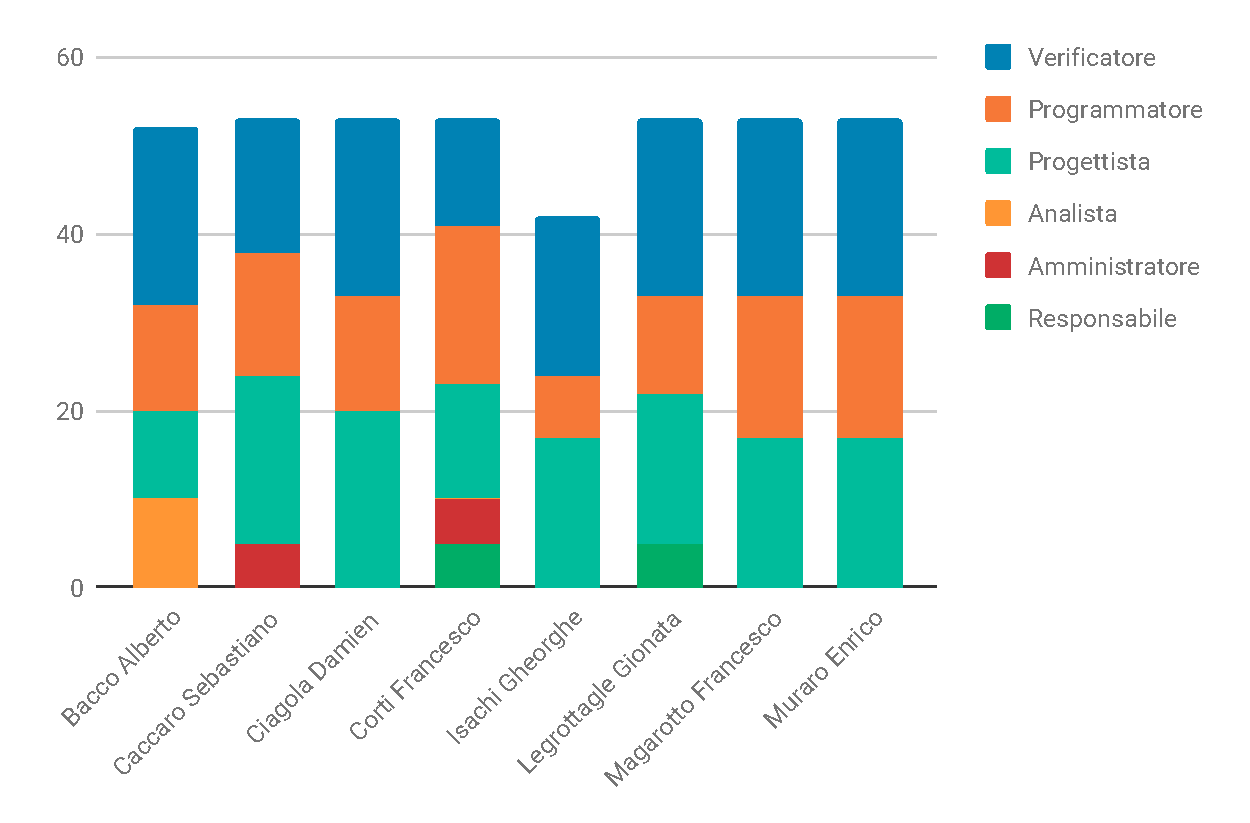
\includegraphics[scale=.8]{Consuntivo/grafici/ConsCod.pdf} 
\caption{Grafico orario per componente a fine periodo}
\end{figure}
\paragraph{Technology Baseline} \mbox{}\\
A seguito della \RP{} il gruppo ha provveduto a implementare una soluzione alternativa rispetto a quella proposta: il database Firestore è stato sostituito con MongoDB, alternativa open-source e pertanto priva di costi di licenza. Tale scelta è conseguente alla richiesta del docente Cardin di collegare il {database}\ped{G} alla backend al fine di ridurre l'accoppiamento. Lo studio di fattibilità di tale soluzione ha portato a complessità inaspettate, soprattutto nella stesura del codice Java, pertanto si è ritenuto opportuno provare ad implementare una nuova soluzione, dopo aver contattato e ottenuto l'approvazione da parte della proponente e dal docente. In considerazione del fatto che entrambi i database sono documentali, pertanto la struttura delle collezioni è pressoché identica, e l'integrazione di Spring con MongoDB supportata dalla libreria Spring Data Mongo ha ridotto drasticamente la complessità del codice necessario, il cambio di tecnologia non ha portato a ritardi.

\paragraph{Analisi dei Requisiti} \mbox{}\\
Il documento ha subito un incremento non pianificato, richiesto dal docente per concludere il documento tale incremento ha richiesto più ore per il ruolo di \ana{} rispetto a quanto preventivato.

\paragraph{Ripianificazione attività future} \mbox{}\\
Il periodo di Verifica e Validazione è stato ripianificato rispettando tre principi:
\begin{enumerate}
\item Ogni componente non può svolgere più di 105 ore nel periodo rendicontato;
\item Il nuovo costo preventivato (3.027,00 \euro) per il periodo di Verifica e Validazione non può far superare la cifra (15.061,00 \euro) per il periodo rendicontato presentata in ingresso alla \RR{}. \\Tali modifiche sono presenti nel preventivo a finire a seguire;
\item Ogni componente deve svolgere ogni ruolo per un minimo di 5 ore.
\end{enumerate}

Al momento attuale, dato il numero dei requisiti obbligatori soddisfatti, considerate le problematiche legate alla presenza di due studenti lavoratori e l'intenzione di due studenti di iniziare il tirocinio dopo il primo esame scritto, il numero di requisiti opzionali soddisfatti in sede di \RA{} potrebbe essere minore di quanto pianificato precedentemente.